% !TeX spellcheck = en_GB
\documentclass[english,11pt,aspectratio=1610,xcolor=table]{beamer}
% !TeX root = ../defense.tex
% packages
\usepackage{babel}
\usepackage[utf8]{inputenc}
\usepackage[scaled=0.86]{beramono}
\usepackage{helvet}
\usepackage[T1]{fontenc}

\usepackage{eurosym}
\usepackage{tabularx}
\usepackage[output-decimal-marker={,},per-mode=symbol,exponent-product={\cdot},retain-unity-mantissa=false]{siunitx}
\usepackage{csquotes}
\usepackage{tikz}
\usepackage{pgfplots}
\usepackage{listings}
\usepackage{mathtools}
\usepackage{textcomp}
\usepackage[version=4]{mhchem}
\usepackage{bm}
\usepackage{tabu}
\usepackage{appendixnumberbeamer}

% tikz libraries
\usetikzlibrary{arrows.meta}
\usetikzlibrary{calc}
\usetikzlibrary{decorations.pathreplacing}
\usetikzlibrary{positioning}
\usetikzlibrary{shapes}

% pgfplots libraries
\usepgfplotslibrary{fillbetween} 
% !TeX root = ../defense.tex
% colors
% tum main colors
\definecolor{tumblue}{RGB}{0, 101, 189}
\definecolor{tumblack}{RGB}{0, 0, 0}
\definecolor{tumwhite}{RGB}{255, 255, 255}

% tum blue tones (shades !85, !70, !55 allowed)
\definecolor{tumdarkerblue}{RGB}{0, 51, 89}
\definecolor{tumdarkblue}{RGB}{0, 82, 147}
\definecolor{tummidblue}{RGB}{0, 115, 207}
\definecolor{tumlightblue}{RGB}{100, 160, 200}
\definecolor{tumlighterblue}{RGB}{152, 198, 234}

% tum grey tones
\definecolor{tumdarkergrey}{RGB}{44, 44, 45}
\definecolor{tumdarkgrey}{RGB}{88, 88, 90}
\definecolor{tumgrey}{RGB}{156, 157, 159}
\definecolor{tumlightgrey}{RGB}{217, 218, 219}
\definecolor{tumlightergrey}{RGB}{235, 236, 237}

% tum accent colors (shades !85, !70, !55 allowed)
\definecolor{tumorange}{RGB}{227,114,34}
\definecolor{tumgreen}{RGB}{162,173,0}
\definecolor{tumivory}{RGB}{218,215,203}

% tum extended palette (shades !85, !70, !55 allowed)
\definecolor{tumviolet}{RGB}{105,8,90}
\definecolor{tumdarkviolet}{RGB}{15,27,95}
\definecolor{tumturquois}{RGB}{0,119,138}
\definecolor{tumdarkgreen}{RGB}{0,124,48}
\definecolor{tummidgreen}{RGB}{103,154,29}
\definecolor{tumbrightyellow}{RGB}{255,220,0}
\definecolor{tumbrightorange}{RGB}{249,186,0}
\definecolor{tumbrightred}{RGB}{214,76,19}
\definecolor{tumred}{RGB}{196,7,27}
\definecolor{tumdarkred}{RGB}{156,13,22}


% tum presentation colors (styleguide, p.266)
\definecolor{tumpyellow}{RGB}{255,180,0}
\definecolor{tumporange}{RGB}{255,128,0}
\definecolor{tumpred}{RGB}{229,52,24}
\definecolor{tumpdarkred}{RGB}{202,33,63}
\definecolor{tumpblue}{RGB}{0,153,255}
\definecolor{tumpbrightblue}{RGB}{65,190,255}
\definecolor{tumpgreen}{RGB}{145,172,107}
\definecolor{tumpbrightgreen}{RGB}{181,202,130}

% custom thesis colors
\definecolor{biomass}{RGB}{0, 122, 55}
\definecolor{co2}{RGB}{160, 160, 160}
\definecolor{coal}{RGB}{100, 100, 100}
\definecolor{cool}{RGB}{0, 0, 255}
\definecolor{demand}{RGB}{25, 25, 25}
\definecolor{diesel}{RGB}{116, 66, 65}
\definecolor{gas}{RGB}{128, 64, 0}
\definecolor{elec}{RGB}{255, 170, 0}
\definecolor{heat}{RGB}{230, 112, 36}
\definecolor{hydro}{RGB}{198, 188, 240}
\definecolor{hydrogen}{RGB}{198, 188, 240}
\definecolor{imp}{RGB}{128, 128, 200}
\definecolor{lignite}{RGB}{116, 66, 65}
\definecolor{nuclear}{RGB}{192, 34, 16}
\definecolor{oil}{RGB}{116, 66, 65}
\definecolor{overproduction}{RGB}{190, 0, 99}
\definecolor{slack}{RGB}{163, 74, 130}
\definecolor{solar}{RGB}{243, 174, 0}
\definecolor{storage}{RGB}{60, 36, 154}
\definecolor{wind}{RGB}{122, 179, 225}
\definecolor{stock}{RGB}{222, 222, 222}

% custom building type colors
\definecolor{basin}{RGB}{110, 75, 56}
\definecolor{chapel}{RGB}{177, 121, 91}
\definecolor{church}{RGB}{177, 121, 91}
\definecolor{commercial}{RGB}{129, 162, 190}
\definecolor{farm}{RGB}{202, 178, 214}
%\definecolor{garage}{RGB}{253, 191, 111}
\definecolor{greenhouse}{RGB}{255, 127, 0}
%\definecolor{hospital}{RGB}{129, 221, 190}
\colorlet{hospital}{tumturquois}
%\definecolor{hotel}{RGB}{227, 26, 28}
\colorlet{hotel}{tumorange!50}
\definecolor{house}{RGB}{181, 189, 104}
\definecolor{industrial}{RGB}{240, 198, 116}
\definecolor{office}{RGB}{129, 162, 190}
%\definecolor{public}{RGB}{129, 162, 190}
\definecolor{residential}{RGB}{181, 189, 104}
\definecolor{restaurant}{RGB}{227, 26, 28}
%\definecolor{retail}{RGB}{129, 162, 190}
\definecolor{school}{RGB}{29, 103, 214}
%\definecolor{warehouse}{RGB}{98, 134, 6}
\colorlet{warehouse}{tumgrey!50}
\colorlet{garage}{tumgrey!75}
\colorlet{public}{commercial!50}
\colorlet{other}{tumgrey}
\colorlet{retail}{commercial!75}


% Pgfplots settings and styles
\pgfplotsset{%
    compat=1.12,
    major grid style={thin, color=gray!25},
    minor grid style={thin, color=gray!25},
    tumaxisstyle/.style={
        axis line style={opacity=0}, major tick style={draw=none},
        ymajorgrids, xmajorgrids},
        every axis/.append style={font=\footnotesize},
        legend style={draw=none, legend cell align=left},
    /pgfplots/square ybar legend/.style={
        /pgfplots/legend image code/.code={%
            \fill[##1,/tikz/.cd,bar width=.5em]
            plot coordinates { (\pgfplotbarwidth,.5em)};}}
}

% Tikz styles
\tikzset{%
    flowbox/.style={rectangle split, rectangle split parts=2, 
                    rectangle split part fill={jddarkblue,jddarkblue!20},
                    align=center},
    conn/.style={draw=jdblue, -{Latex[length=3mm]}, 
                 rounded corners=3pt},
    hidden/.style={-{Latex[length=2mm]}, draw=tumdarkgrey,
                   rounded corners=2pt, densely dotted},
    concept/.style={fill=jddarkgrey!15},
    darrows/.style={{Latex[length=2mm]}-{Latex[length=2mm]}},
    onslide/.code args={<#1>#2}{\only<#1>{\pgfkeysalso{#2}}},
    fb-muted/.style={rectangle split part fill={jdgrey,jdgrey!15}},
    fb-highlight/.style={rectangle split part fill={jdgreen,jdgreen!20}}
}

% Tikz commands
\newcommand{\fbtitle}[1]{\textbf{\textcolor{jdwhite}{#1}}}

% custom units for siunitx
\DeclareSIUnit\year{a}
\DeclareSIUnit\billion{$\!$b}
\DeclareSIUnit\million{$\!$m}
\DeclareSIUnit\thousand{$\!$k}
\DeclareSIUnit\USD{\$}
\DeclareSIUnit\EUR{\text{\euro}}
\DeclareSIUnit\kWp{kW$\!_p$}
\DeclareSIUnit{\TWh}{TWh}
\DeclareSIUnit{\GWh}{GWh}
\DeclareSIUnit{\MWh}{MWh}
\DeclareSIUnit{\TW}{\tera\watt}
\DeclareSIUnit{\hectar}{ha}
\AtBeginDocument{\DeclareSIUnit{\kWh}{kWh}}

% handy commands
\newcommand{\bs}{\boldsymbol}
\newcommand{\st}{\mathsf{s.t.}}
\newcommand{\R}{\mathbb{R}}
\newcommand{\Z}{\mathbb{Z}}
\newcommand{\T}{^\mathsf{T}}
\newcommand{\scenario}[1]{\textcolor{jdgreen}{#1}}

% beamer dimensions
\newlength{\maxheight}
\setlength{\maxheight}{\textheight}
\addtolength{\maxheight}{-\headheight}
\addtolength{\maxheight}{-\footheight}
\addtolength{\maxheight}{-2em} % guessing :-(

\AtBeginDocument{%
\newlength{\squeezetwo}
\setlength{\squeezetwo}{.495\paperwidth}
%
\newlength{\squeezethree}
\setlength{\squeezethree}{.33\paperwidth}
%
\newlength{\loosethree}
\setlength{\loosethree}{.29\textwidth}
}

% listings settings
\lstset{
    basicstyle={\color{jddarkgrey}\ttfamily},
    identifierstyle=\color{jddarkblue},
    commentstyle={\color{jdgreen}},
    stringstyle={\color{gred}},
    keywordstyle={\color{jddarkerblue}},
    emphstyle={\color{jdlightblue}},
    emph={urbs,rivus},
    texcl=true
}

% hyperref settings
\hypersetup{colorlinks=true,linkcolor=,urlcolor=jdgreen}


\usetheme{JD}
\beamertemplatenavigationsymbolsempty

% header fields: usage
% \field
%     [short form (footline)]
%     {long form on title page}
%
\title
    [Using Past Speaker Behavior to Better Predict Turn Transitions]
    {Using Past Speaker Behavior to Better Predict Turn Transitions}

\subtitle{Thesis Presentation} % short version unused by this template
\author
    [T. Meshorer]
    {Tomer Meshorer}
\institute
    [\hypersetup{urlcolor=jdgrey}%
     \href{http://www.ohsu.edu/}{OHSU} ]
    {Center for Spoken Language Understanding\\
     Oregon Health \& Science University\\
     Portland, Oregon,USA}
\date
    [06/2017]
    {08 June 2017}

\begin{document}

\maketitle

\begin{frame}{Outline}
    \tableofcontents
\end{frame}

`% !TeX root = ../defense.tex

\section{Motivation}
\frame{\sectionpage}




\begin{frame}{Current Issues}
    \begin{enumerate}
      \item For a natural conversation between human and machine, we want to conform
            to human to human turn taking system (Sacks et al, 1974)
                \begin{itemize}
                    \item One speaker at the time
                    \item Overlap speech is common but brief (only 17% of turns, 100ms long)
                    \item Gaps between turns kept to a minimum (200 ms)
                    \item No fixed turn size and no fixed conversation size.
                \end{itemize}
      \item In Human-Human conversations conversants predict (Sacks et al, 1974) or
            signal (Duncan 1972) each other on coming turn transition
      \item Spoken Dialogue Systems mainly use time-out for predicting turn transition.      
      \item {
        However, timeouts leads to poor user interaction(Arsikere et al, 2015)
        \begin{itemize}
            \item Not effective in noisy environment
            \item Too little - machine barge in during intra turn pause.
            \item Too much - user waiting for the machine.
        \end{itemize}
      }
      \item {
        Recent research tries to use utterance's local features but still do not match human performance.
        \begin{itemize}
            \item Syntactic (Sacks et al 1978,De Ruiter et al. 2006)
            \item Prosodic (Ford 1996,Stolcke 2002,Ferrer 2003)
            \item Pragmatic (Ford 2001)
        \end{itemize}
      }
    \end{enumerate}
\end{frame}

\begin{frame} {Thesis Statement}
   \begin{enumerate}
         \item Conversant's past behavior can help predict turn transitions
         \item Past behavior is represented by summary features
         \begin{itemize}
            \item {\em Relative turn length}: current turn length so far (in seconds and words) relative to the speaker's average turn length
            \item {\em Relative Floor Control}: the speaker's control of the conversation floor (in seconds and words) relative to the total conversation length
         \end{itemize}
         \item Computed for each dialog act.
     \end{enumerate}
 \end{frame} 
 
`% !TeX root = ../defense.tex

\section{Related Work}
\frame{\sectionpage}


\begin{frame}{Turn taking in human-human conversations}
    \begin{enumerate}
       \item (Duncan 1972) Some signals and rules for taking speaking turns in conversations
          \begin{itemize}
            \item Intonation : terminate the final clause with rising or falling pitch.
            \item Drawl on the final syllable
            \item Body motion,
            \item Sociocentric sequence ("you know")
            \item Drop in pitch or loudness
            \item Syntax - completion of grammatical clause , involving subject-predicate combination.
          \end{itemize}
       \item (Sacks et al, 1974) A Simplest Systematics for the Organization of Turn-Taking for Conversation
          \begin{itemize}
            \item Introduced Turn Construction Unit (TCU) (word, phrase, clause, sentence)
            \item Defined Transition Relevance Place (TRP) between TCUs. Defined a local turn allocation system which is operational in each TRP
            \begin{itemize}
                \item Current speaker selects the next conversant;
                \item If the current speaker did not select, any of the listeners can self select; or
                \item If neither of the previous two cases apply, the current speaker continue.
            \end{itemize}
          \end{itemize}
       \item Later research focused on local features
        \begin{itemize}
            \item Syntactic (Sacks et al 1978,De Ruiter et al. 2006)
            \item Prosodic (Ford 1996,Stolcke 2002,Ferrer 2003)
            \item Pragmatic (Ford 2001)
        \end{itemize}
    \end{enumerate}
\end{frame}

\begin{frame} {Turn taking in Spoken dialogue systems I }
   \begin{enumerate}
         \item Early systems used time out based on speech signal threshold. Fixed length of 500ms (Arsikere et al, 2015)
         \item A. Raux and M. Eskenazi. (2009) - A Finite-State Turn-Taking Model for Spoken Dialog System
             \begin{itemize}
                \item Used a 6 state non deterministic state machine to model the turn taking system between the user and the system.
                \item Define a set of possible actions that both user and the system can take:
                      Grab the floor, Release the floor, Wait while not claiming the floor, and Keep
                      the floor.   
                \item Created a cost matrix to assign cost to each action in the state machine.
                \item Applied probabilistic decision theory principle of selecting the action with lowest expected cost
                \item Improvement of 29.5\% over the fixed timeout.    
             \end{itemize}  
         \item Selfridge and Heeman (2010) - A Bidding Approach to Turn-Taking
         \begin{itemize}
            \item Utterance importance is a driving force behind turn-taking
            \item Conversant measures the importance of their potential contribution when negotiating
                  the right to the conversation floor.
            \item Use Reinforcement Learning to map a given situation to the optimal utterance and bidding behavior  
             \item In relation to our work, conversants might use summary feature to signal their bid.        
         \end{itemize}
                 
   \end{enumerate}
 \end{frame}

\begin{frame} {Turn taking in Spoken dialogue systems II }
   \begin{enumerate}
      \item Gravano and Hirschberg (2011) - Turn-taking cues in task-oriented dialogue
         \begin{itemize}
            \item Impressive study of local utterance features as cues (signals) for turn taking.
            \item Formalized and verified Ducan work on signaling.
            \item Defined an IPU - Inter Pausal Unit. Max Sequence of words surrounded by silence.
            \item Tested over 200 features.  prosodic , syntactic , IPU duration, speaking rate.
            \item Found the combining features can improve turn transition prediction.
            \item Our work can complement the local features.
         \end{itemize}
        
         \item N. Guntakandla and R. Nielsen (2015) - Modelling turn-taking in human conversations
         \begin{itemize}
            \item Used dialog act as local feature.
            \item Tested prediction based on Bigram, Trigram and 4-gram of dialog acts.
            \item We based our base models on current and previous dialog acts.
            \item We used the same corpus, but mapped the dialog act types from 148 to 9.
         \end{itemize}
   \end{enumerate}
 \end{frame}


`% !TeX root = ../defense.tex

\section{Theoretical Model}
\frame{\sectionpage}

\begin{frame}{Relative Turn Length}{Timing Diagram}
\begin{center}
\begin{tikzpicture}
 %   \begin{axis}[
 %       tumaxisstyle,
 %       x post scale=1.75,
     %   ymin=0,ymax=3,
 %        xmin=0,xmax=24,
 %        xlabel={Time}]
     %   ylabel={Turns}]
 %    \end{axis}
    \draw [->, thick, black] (0,0) -- (12.5,0);
    \draw (0,-.2) -- (0, .2);
    \draw (0.5,-.2) -- (0.5, .2);
    \draw (1,-.2) -- (1, .2);
    \draw (1.5,-.2) -- (1.5, .2);
    \draw (2,-.2) -- (2, .2);
    \draw (2.5,-.2) -- (2.5, .2);
    \draw (3,-.2) -- (3, .2);
    \draw (3.5,-.2) -- (3.5, .2);
    \draw (4,-.2) -- (4, .2);
    \draw (4.5,-.2) -- (4.5, .2);
    \draw (5,-.2) -- (5, .2);
    \draw (5.5,-.2) -- (5.5, .2);
    \draw (6,-.2) -- (6, .2);
    \draw (6.5,-.2) -- (6.5, .2);
    \draw (7,-.2) -- (7, .2);
    \draw (7.5,-.2) -- (7.5, .2);
    \draw (8,-.2) -- (8, .2);
    \draw (8.5,-.2) -- (8.5, .2);
    \draw (9,-.2) -- (9, .2);
    \draw (9.5,-.2) -- (9.5, .2);
    \draw (10,-.2) -- (10, .2);
    \draw (10.5,-.2) -- (10.5, .2);
    \draw (11,-.2) -- (11, .2);
    \draw (11.5,-.2) -- (11.5, .2);
    \draw (12,-.2) -- (12, .2);

    \draw (17,-.2) -- (17, .2);

    \node at (-1,-0.5) {Time};
    \node at (0,-0.5) {0};
    \node at (1,-0.5) {1};
    \node at (2,-0.5) {2};
    \node at (3,-0.5) {3};
    \node at (4,-0.5) {4};
    \node at (5,-0.5) {5};
    \node at (6,-0.5) {6};
    \node at (7,-0.5) {7};
    \node at (8,-0.5) {8};
    \node at (9,-0.5) {9};
    \node at (10,-0.5) {10};
    \node at (11,-0.5) {11};
    \node at (12,-0.5) {12};

    \node at (-1,1) {A};
    \node at (-1,2.5) {B};

    %A turn 1 , 0 - 1.5 sec with one da
    \uncover<1->{%
      \path [fill=gray] (0,0.5) rectangle (1.5,1.5);
    }

    \uncover<2->{%
        \draw [<->] (0,2.2) -- node[above] {T1} (1.5,2.2);
        \draw [<->] (0,1.6) -- node[above] {da1} (1.5,1.6);
    }

    %B turn 1, da1  2 - 3
    \uncover<3->{%
       \path [fill=teal] (2,2) rectangle (3,3);
       \draw [<->] (2,3.2) -- node[above] {da1} (3,3.2);
       \draw [->]  (0,6) node [left] {Transition} -- (1.8,2.3);

    }


    %B turn 1, da2 3.2 - 4
    \uncover<4->{%
        \path [fill=teal] (3.2,2) rectangle (4,3);
        \draw [<->] (3.2,3.2) -- node[above] {da2} (4,3.2);
    }

    \uncover<5->{%
            \draw [<->] (2,4) -- node[above] {T1} (4,4);
    }


    % A turn 2 4.5 - 6
    \uncover<6->{%
       \path [fill=gray] (4.5,0.5) rectangle (6,1.5);
    }

    % A turn 2 4.5 - 6 , header
    \uncover<7->{%
        \draw [<->] (4.5,2.2) -- node[above] {T2} (6,2.2);
        \draw [<->] (4.5,1.6) -- node[above] {da2} (6,1.6);
    }


    %B turn 2 6.5 - 7.5
    \uncover<8->{%
       \path [fill=teal] (6.5,2) rectangle (7.5,3);
    }

    %B turn 2 6.5 - 7.5 header
    \uncover<9->{%
        \draw [<->] (6.5,3.2) -- node[above] {da3} (7.5,3.2);
        \draw [<->] (6.5,4) -- node[above] {T2=1 sec} (7.5,4);
    }

    %A turn 3, da3=0.5, avg turn length: 1.5, RTL = 0.5/1.5
    \uncover<10->{%
       \path [fill=gray] (8,0.5) rectangle (8.5,1.5);
       \draw [<->] (8,1.6) -- node[above] {da3} (8.5,1.6);

    }

    \only<10> {
       \node at (11,3) {\small{Avg Turn Length: 1.5}};
       \node at (11,3.5) {\small{Relative Turn Length: $33\%$}};
       \draw [<->] (8,2.2) -- node[above] {\small{0.5 sec}} (8.5,2.2);
    }

    %A turn 3, da4, avg turn length: 1.5, RTL = 2/1.5
    \uncover<11->{%
       \path [fill=gray] (8.7,0.5) rectangle (10.3,1.5);
       \draw [<->] (8.7,1.6) -- node[above] {da4} (10.3,1.6);
    }

    \only<11> {
       \node at (11,3) {\small{Avg Turn Length: 1.5}};
       \node at (11,3.5) {Relative Turn Length: $153\%$};
       \draw [<->] (8,2.2) -- node[above] {\small{2.3 sec}} (10.3,2.2);

    }


    \uncover<12->{% avg turn length: 1.5, RTL = 3/1.5
       \path [fill=gray] (10.5,0.5) rectangle (11.5,1.5);
       \draw [<->] (10.5,1.6) -- node[above] {da5} (11.5,1.6);
    }

    \only<12> {
       \node at (11,3) {\small{Avg Turn Length: 1.5}};
       \node at (11,3.5) {Relative Turn Length: $233\%$};
       \draw [<->] (8,2.2) -- node[above] {\small{3.5 sec}} (11.5,2.2);

    }

\end{tikzpicture}
\end{center}
\end{frame}




\begin{frame}{Relative Floor Control}{Timing Diagram}
\begin{center}
\begin{tikzpicture}
 %   \begin{axis}[
 %       tumaxisstyle,
 %       x post scale=1.75,
     %   ymin=0,ymax=3,
 %        xmin=0,xmax=24,
 %        xlabel={Time}]
     %   ylabel={Turns}]
 %    \end{axis}
    \draw [->, thick, black] (0,0) -- (12.5,0);
    \draw (0,-.2) -- (0, .2);
    \draw (0.5,-.2) -- (0.5, .2);
    \draw (1,-.2) -- (1, .2);
    \draw (1.5,-.2) -- (1.5, .2);
    \draw (2,-.2) -- (2, .2);
    \draw (2.5,-.2) -- (2.5, .2);
    \draw (3,-.2) -- (3, .2);
    \draw (3.5,-.2) -- (3.5, .2);
    \draw (4,-.2) -- (4, .2);
    \draw (4.5,-.2) -- (4.5, .2);
    \draw (5,-.2) -- (5, .2);
    \draw (5.5,-.2) -- (5.5, .2);
    \draw (6,-.2) -- (6, .2);
    \draw (6.5,-.2) -- (6.5, .2);
    \draw (7,-.2) -- (7, .2);
    \draw (7.5,-.2) -- (7.5, .2);
    \draw (8,-.2) -- (8, .2);
    \draw (8.5,-.2) -- (8.5, .2);
    \draw (9,-.2) -- (9, .2);
    \draw (9.5,-.2) -- (9.5, .2);
    \draw (10,-.2) -- (10, .2);
    \draw (10.5,-.2) -- (10.5, .2);
    \draw (11,-.2) -- (11, .2);
    \draw (11.5,-.2) -- (11.5, .2);
    \draw (12,-.2) -- (12, .2);

    \draw (17,-.2) -- (17, .2);

    \node at (-1,-0.5) {Time};
    \node at (0,-0.5) {0};
    \node at (1,-0.5) {1};
    \node at (2,-0.5) {2};
    \node at (3,-0.5) {3};
    \node at (4,-0.5) {4};
    \node at (5,-0.5) {5};
    \node at (6,-0.5) {6};
    \node at (7,-0.5) {7};
    \node at (8,-0.5) {8};
    \node at (9,-0.5) {9};
    \node at (10,-0.5) {10};
    \node at (11,-0.5) {11};
    \node at (12,-0.5) {12};

    \node at (-1,1) {A};
    \node at (-1,2.5) {B};

    %A turn 1 , 0 - 1.5 sec with one da
    \uncover<1->{%
      \path [fill=gray] (0,0.5) rectangle (1.5,1.5);
      \draw [<->] (0,2.2) -- node[above] {T1} (1.5,2.2);
      \draw [<->] (0,1.6) -- node[above] {da1} (1.5,1.6);
    % B Trun  
      \path [fill=teal] (2,2) rectangle (3,3);
      \draw [<->] (2,3.2) -- node[above] {da1} (3,3.2);
      \path [fill=teal] (3.2,2) rectangle (4,3);
      \draw [<->] (3.2,3.2) -- node[above] {da2} (4,3.2);
      \draw [<->] (2,4) -- node[above] {T1} (4,4);
    }

    %Total Length
    \only<1> {
        \node at (11,4) {\small{A RTC: 42\%}};
        \node at (11,3) {\small{B RTC: 58\%}};
        \draw [<->] (0,4.7) -- node[above] {\small{A: 1.5 secs / B: 2 secs}} (4,4.7);
    }

    % A turn 2 4.5 - 6
    \uncover<2->{%
       \path [fill=gray] (4.5,0.5) rectangle (6,1.5);
       \draw [<->] (4.5,2.2) -- node[above] {T2} (6,2.2);
       \draw [<->] (4.5,1.6) -- node[above] {da2} (6,1.6);
    }

    %Total Length
    \only<2> {
        \node at (11,4) {\small{A RTC: 60\%}};
        \node at (11,3) {\small{B RTC: 40\%}};
        \draw [<->] (0,4.7) -- node[above] {\small{A: 3 secs / B: 2 secs}} (6,4.7);
    }

    %B turn 2 6.5 - 7.5
    \uncover<3->{%
       \path [fill=teal] (6.5,2) rectangle (7.5,3);
       \draw [<->] (6.5,4) -- node[above] {T2} (7.5,4);
    }

        %Total Length
    \only<3> {
        \node at (11,4) {\small{A RTC: 50\%}};
        \node at (11,3) {\small{B RTC: 50\%}};
        \draw [<->] (0,4.7) -- node[above] {\small{A: 3 secs / B: 3 secs}}  (7.5,4.7);
    }


    %A turn 3, da3=0.5, avg turn length: 1.5, RTL = 0.5/1.5
    \uncover<4->};
        \node at (11,3) {\small{B RTC: 46\%}};
        \draw [<->] (0,4.7) -- node[above] {\small{A: 3.5 secs / B: 3 secs}} (8.5,4.7);
    }

    %A turn 3, da4, avg turn length: 1.5, RTL = 2/1.5
    \uncover<5->};
        \node at (11,3) {\small{B RTC: 37.5\%}};
        \draw [<->] (0,4.7) -- node[above] {\small{A: 5 secs / B: 3 secs}} (10.3,4.7);
    }


    \uncover<6->};
       \node at (11,3) {\small{B RTC: 33\%}};
       \draw [<->] (0,4.7) -- node[above] {\small{A: 6 secs / B: 3 secs}} (11.5,4.7);
    }

\end{tikzpicture}
\end{center}
\end{frame}

`% !TeX root = ../defense.tex

\section{Data Preparation}
\frame{\sectionpage}


\begin{frame}{Corpus}
    \begin{enumerate}[<+->]\itemsep9pt
      \item Switchboard corpus . Originally recorded in 1991. 
      \item Audio recording of casual conversations between randomly chosen speakers.
      \item 2483 conversation, involving 520 speakers
      \item In our research we used the NXT version (S. Calhoun, 2010) of the corpus which contain 642 annotated conversations (XML)
    \end{enumerate}

\end{frame}{}


\begin{frame}{Preprocessing pipeline}
\begin{figure}[ht!]
\centering
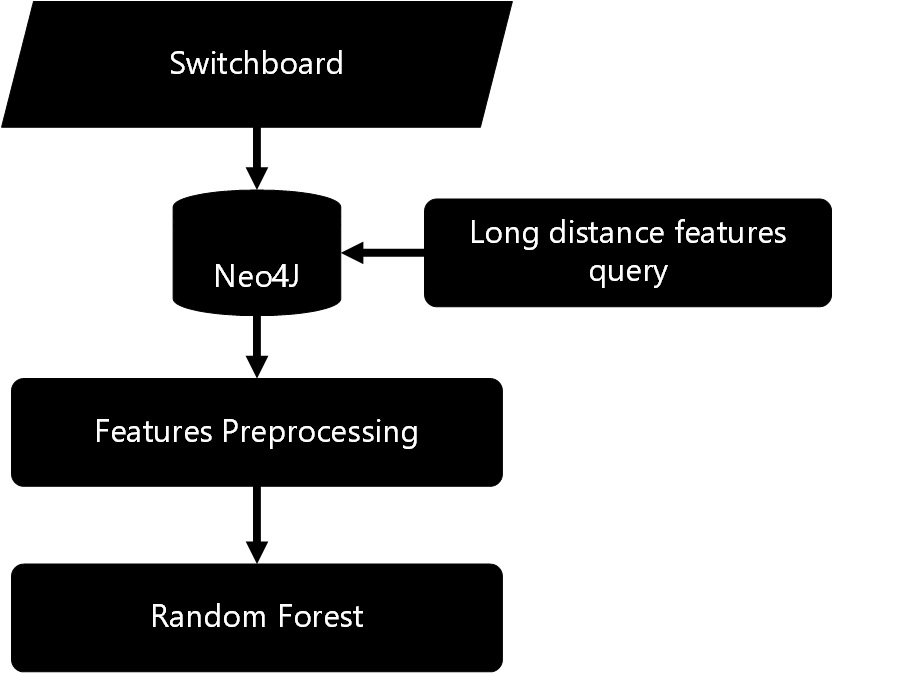
\includegraphics[width=20em]{../latex/pipeline.jpg}\vspace{-1em}
\end{figure}
\end{frame}


\begin{frame}{Conversation representation}
\begin{figure}[ht!]
\centering
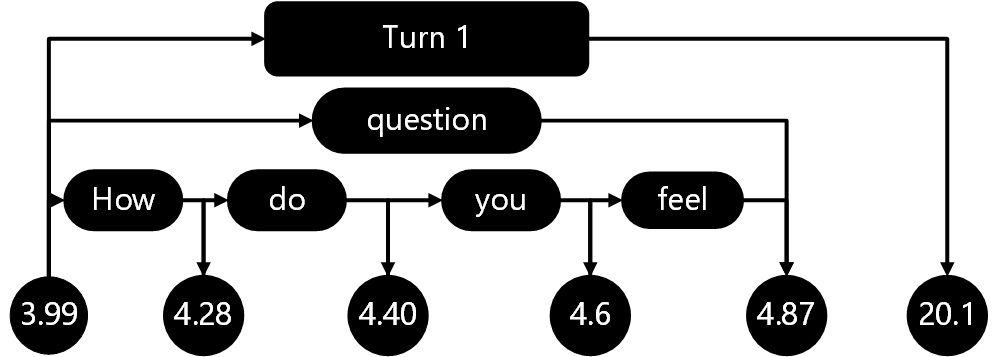
\includegraphics[width=30em]{../latex/graph5.jpg}\vspace{-1em}
\end{figure}
\end{frame}



\begin{frame}{Preprocessing}
 \begin{itemize}
    \item Removed 11 dialogue acts that were coded as other in switchboard.
    \item Reduce data sparsity by collapsing 65 dialog acts into 9.
    \item Performed using python-pandas.
  \end{itemize}

  \begin{table}
     \begin{center}
     \begin{tabular}{l | l}
    \hline
Switchboard dialog acts &  Dialog act classes  \\
    \hline
sd,h,bf      & statement   \\
sv,ad,sv@    & statement - opinion  \\
aa,aa\^r     & agree accept \\
\%.\%-,\%@   & abandon      \\
b,bh         & backchannel  \\
qy,qo,qh     & question     \\
no,ny,ng,arp & answer       \\
+            & +            \\
o@,+@        & NA           \\
  \hline
\end{tabular}
\end{center}\vspace{-0.5em}
\caption{Mapping from dialog act to dialog act class}
\label{tab:mapping}
\end{table}

\end{frame}{}


\section{Data Exploration}
\frame{\sectionpage}

\begin{frame}{Overview}
     \begin{enumerate}[<+->]\itemsep9pt
          \item Want to understand distribution of the input variables.
          \item Want to understand correlations between the input features and outcome (turn transition)
          \item Done using python pandas for data preparation and python seaborn for data visualization
      \end{enumerate}
\end{frame}


\begin{frame}{Dialog act relative count}
\begin{minipage}{0.8\textwidth}
\begin{figure}[H]
\centering
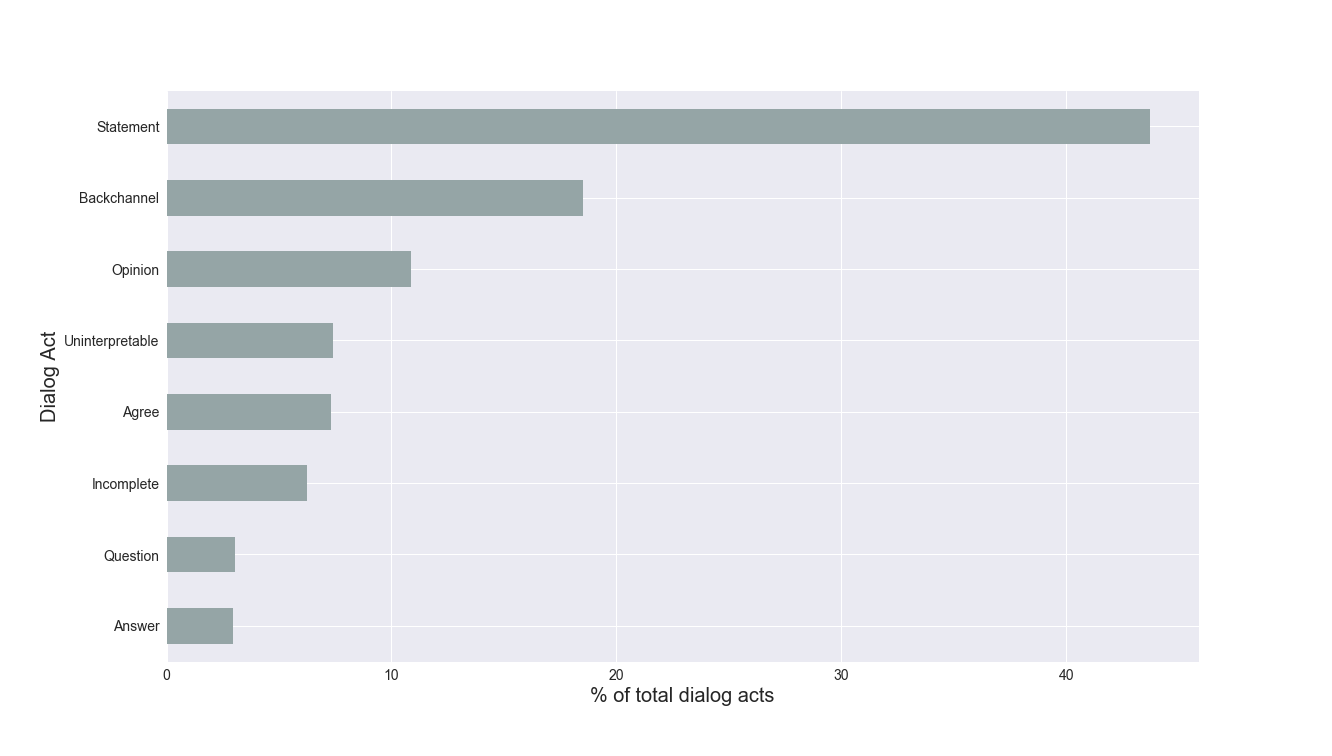
\includegraphics[width=30em]{../scikitlearn/figures/f1.png}
\end{figure}
\end{minipage}
\begin{minipage}{0.8\textwidth}
\begin{itemize}
\item Mainly Statements and Backchannels.
\item Representative of casual conversations.
\end{itemize}
\end{minipage}
\end{frame}

\begin{frame}{Turn Length Distribution}
\begin{minipage}{0.8\textwidth}
\begin{figure}[H]
\centering
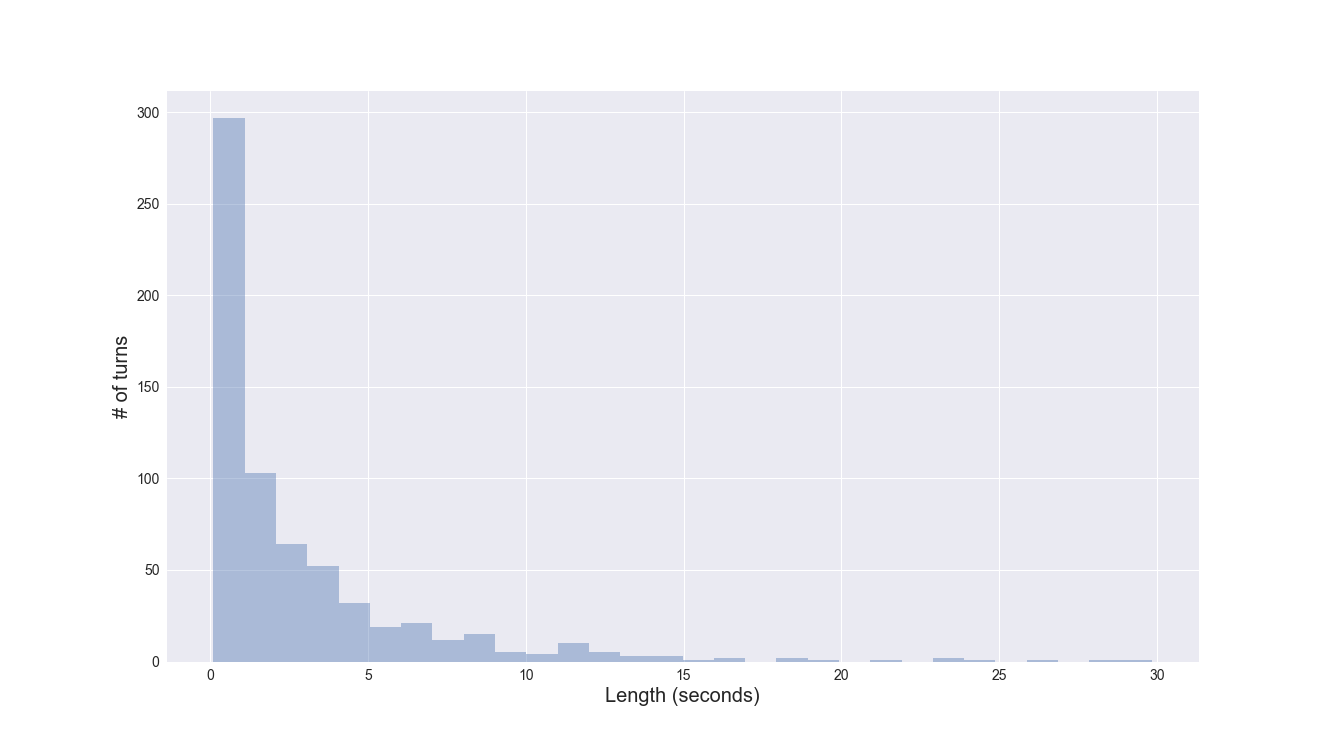
\includegraphics[width=30em]{../scikitlearn/figures/f10.png}\vspace{-1em}
\end{figure}
\end{minipage}
\begin{minipage}{0.8\textwidth}
\begin{itemize}
\item \small{Very skewed distribution}
\item \small{Long flat tail}
\end{itemize}
\end{minipage}
\end{frame}



\begin{frame}{Dialog act probability of turn change}
\begin{minipage}{0.8\textwidth}
\begin{figure}[H]
\centering
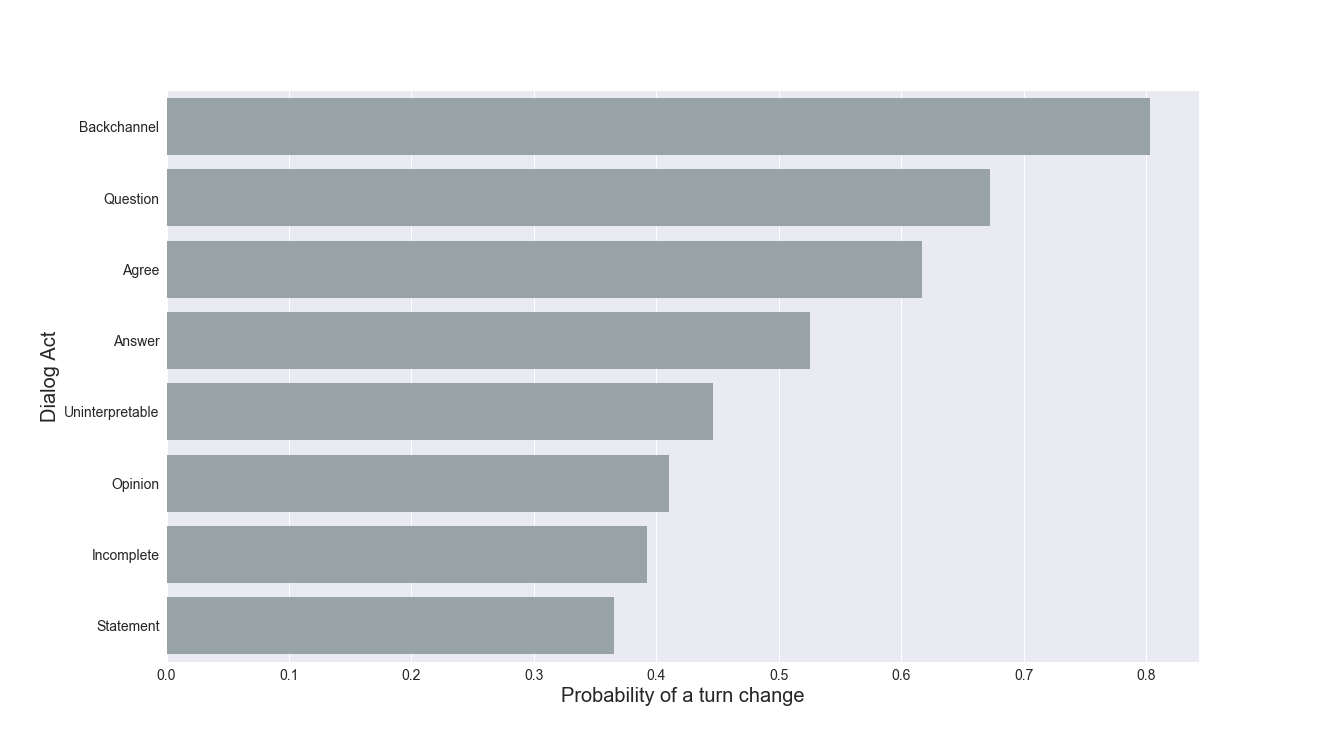
\includegraphics[width=30em]{../scikitlearn/figures/f2.png}\vspace{-1em}
\end{figure}
\end{minipage}
\begin{minipage}{0.8\textwidth}
\begin{itemize}
\item \small{Backchannels mostly leads to turn change (Explain the previous slide)}
\end{itemize}
\end{minipage}
\end{frame}



\begin{frame}{Relative Turn Length effect on probability of turn change}
\begin{minipage}{0.8\textwidth}
\begin{figure}[H]
\centering
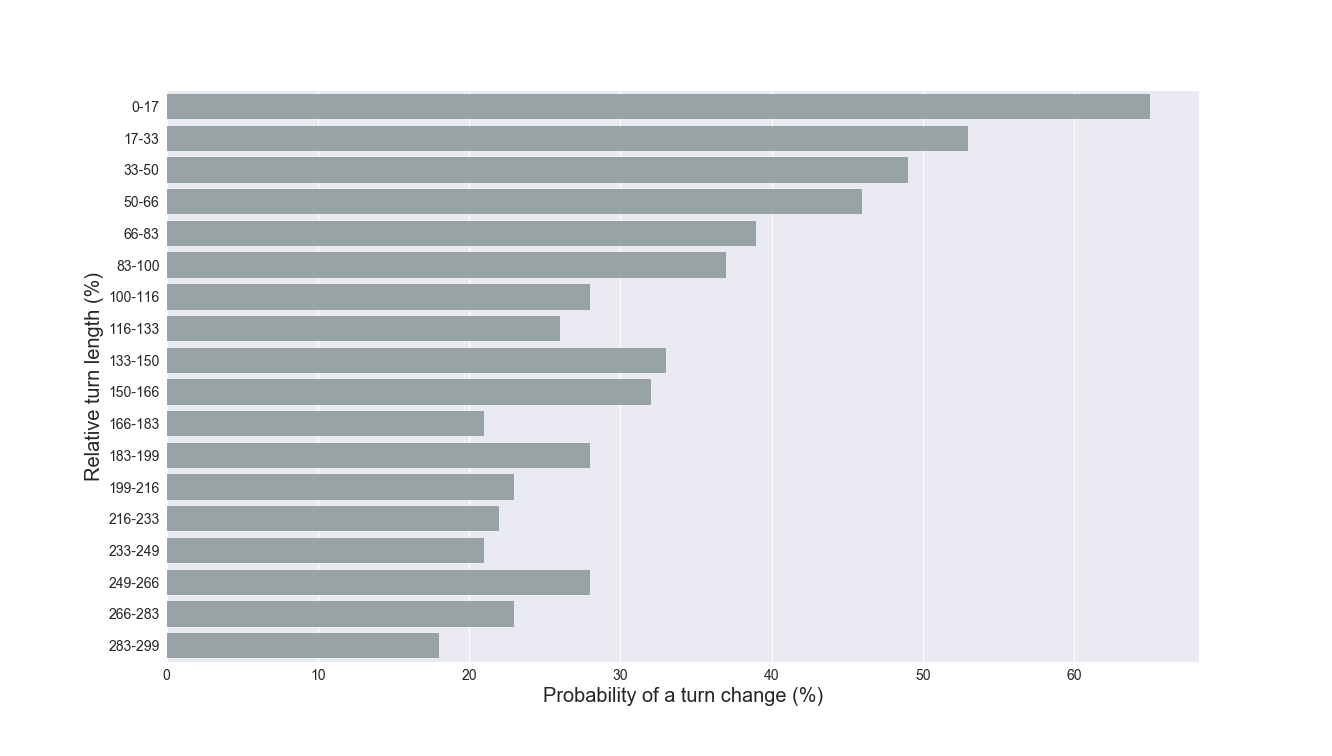
\includegraphics[width=36em]{../scikitlearn/figures/f5.png}\vspace{-1em}
\end{figure}
\end{minipage}
\begin{minipage}{0.8\textwidth}
\begin{itemize}
\item \small{Dialog act with small relative length lead to turn change.}
\item \small{As the speaker has the floor for more time, the speaker tends to hold it.}
\end{itemize}
\end{minipage}
\end{frame}

\begin{frame}{Relative Turn Control effect on probability of a turn change}
\begin{minipage}{0.8\textwidth}
\begin{figure}[H]
\centering
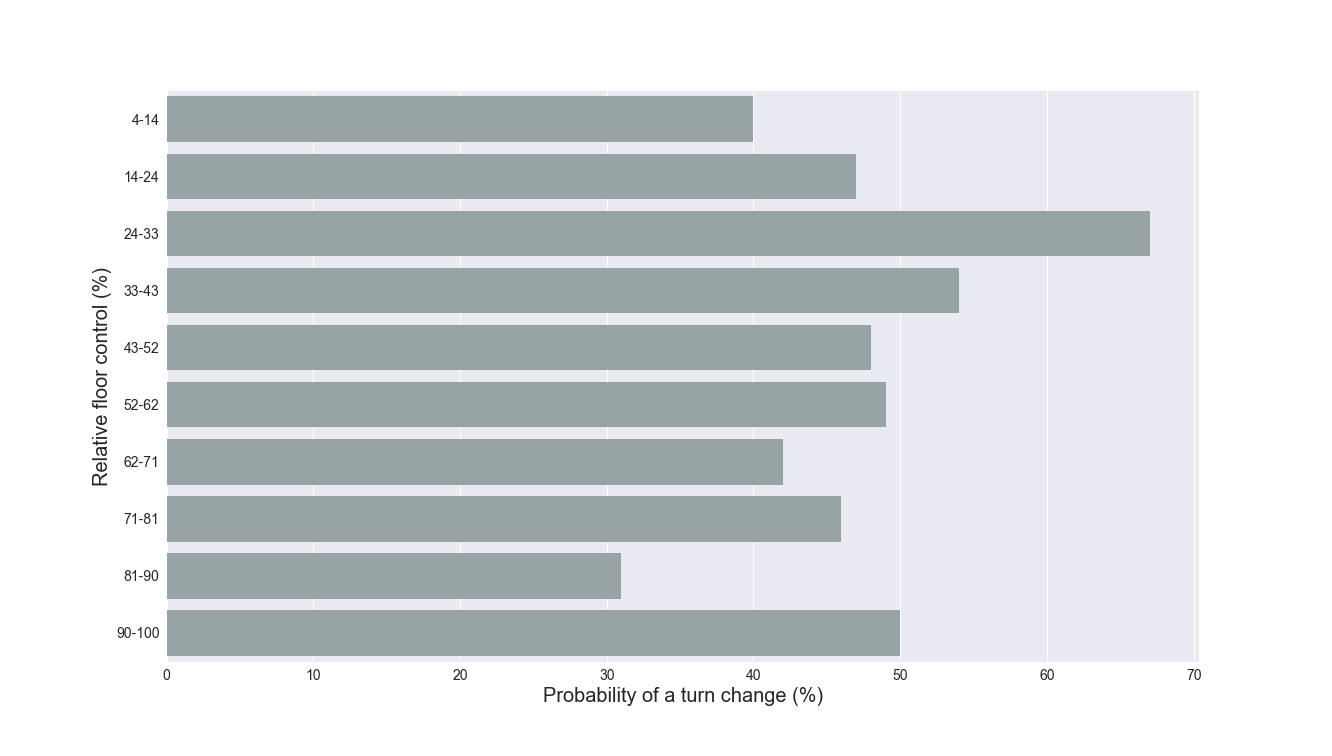
\includegraphics[width=30em]{../scikitlearn/figures/f6.png}\vspace{-1em}
\end{figure}
\end{minipage}
\begin{minipage}{0.8\textwidth}
\begin{itemize}
\item \small{High values of floor control correlate with the willingness of the current speaker to give up the floor.}
\end{itemize}
\end{minipage}
\end{frame}

\begin{frame}{Relative turn length for dialog act type}
\begin{minipage}{0.8\textwidth}
\begin{figure}[H]
\centering
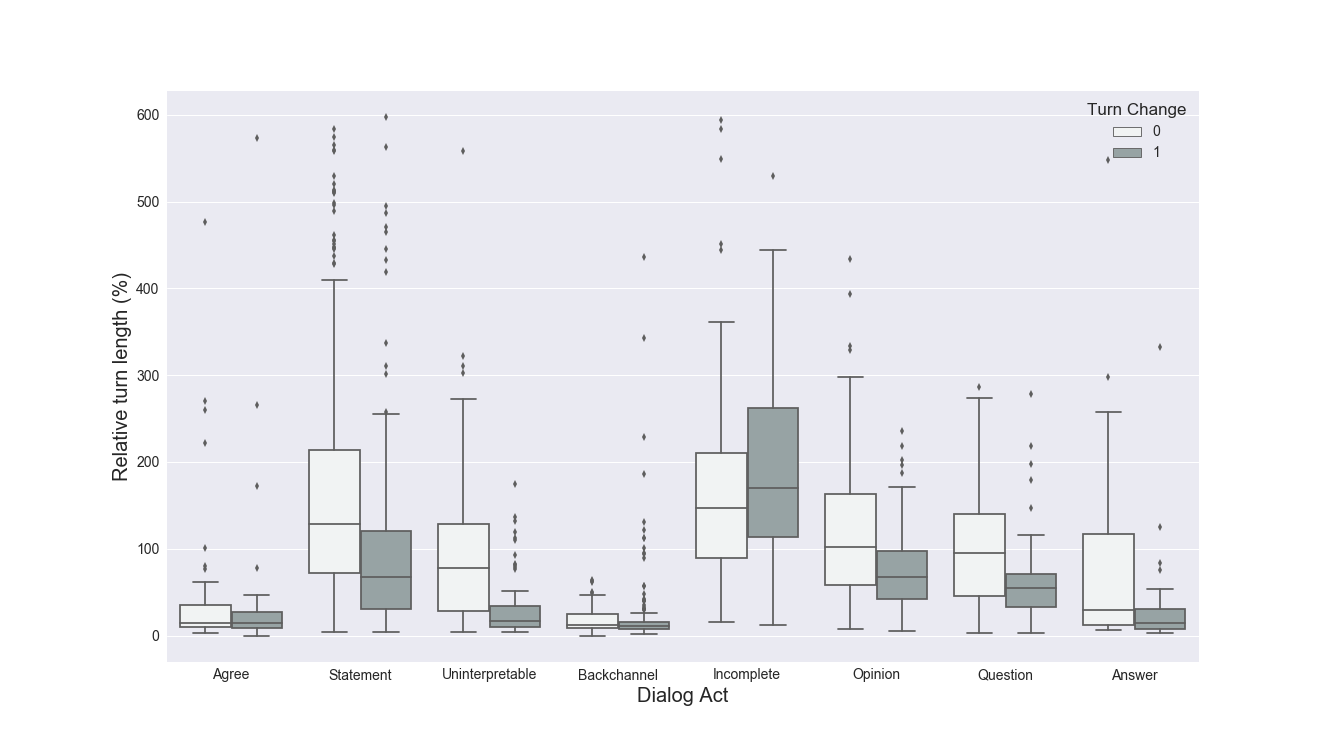
\includegraphics[width=30em]{../scikitlearn/figures/f3.png}\vspace{-1em}
\end{figure}
\end{minipage}
\begin{minipage}{0.8\textwidth}
\begin{itemize}
\item \small{The median relative turn length that led to a turn change is smaller than when it does not.}
\item \small{High RTL do not lead to turn change. Holds across dialog acts} 
\end{itemize}
\end{minipage}
\end{frame}


\begin{frame}{Relative floor control by dialog act}
\begin{minipage}{0.8\textwidth}
\begin{figure}[H]
\centering
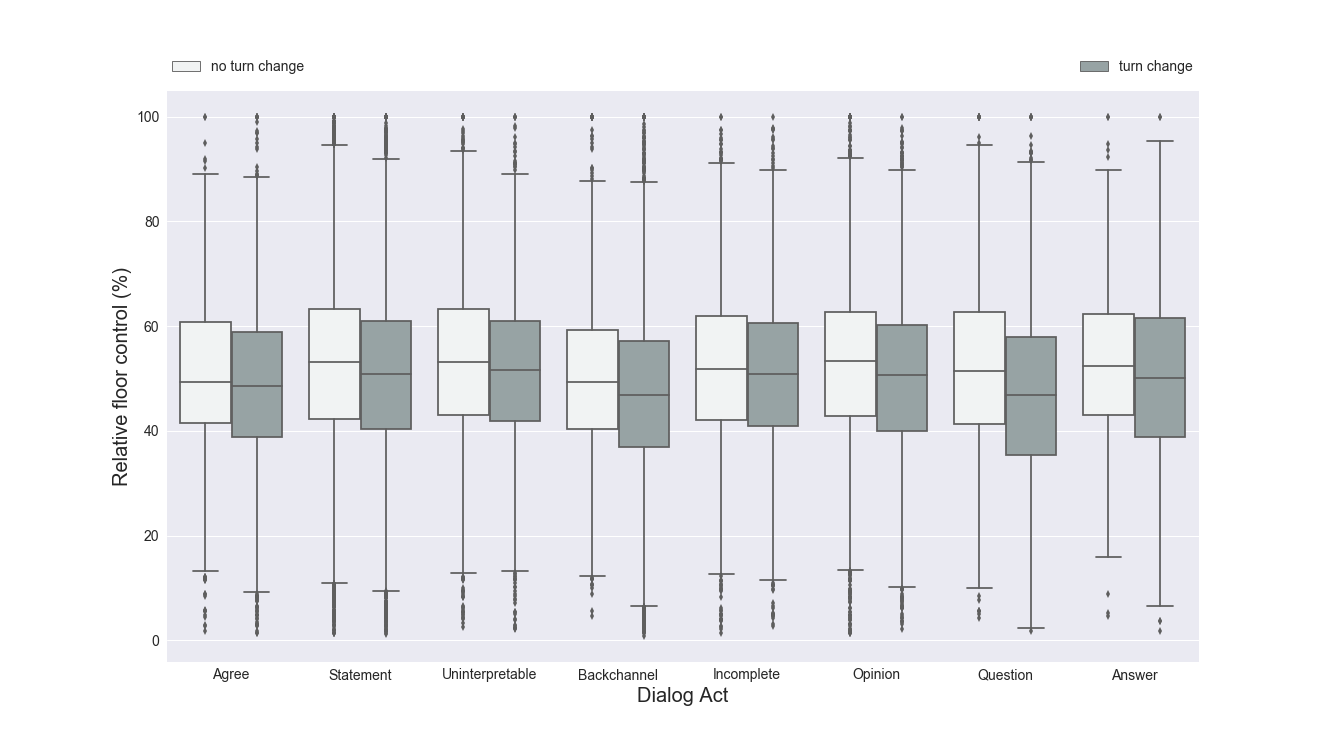
\includegraphics[width=30em]{../scikitlearn/figures/f4.png}\vspace{-1em}
\end{figure}
\end{minipage}
\begin{minipage}{0.8\textwidth}
\begin{itemize}
\item \small{The median is mainly 50\% across dialog acts}
\item \small{The median for relative floor control is slightly higher for each
dialogue act when it not followed by a turn change, than when it is}
\end{itemize}
\end{minipage}
\end{frame}


\begin{frame}{Exploration Summary}
 \begin{enumerate}[<+->]\itemsep9pt
          \item The chance of turn change is higher when the speaker has the floor for shorter than its average turn
          \item Contradict our initial assumption (that high RTL will lead to turn change)
          \item Possible explanation
                \begin{itemize}
                    \item for small relative turn length, this is due to short turn with single dialog act which is likely to be back channel or an answer, both of which have low relative
                     \item for high relative turn length, we attribute to the flat tail of turn length distribution - the chance that the current dialog act will lead to a turn change are smaller and smaller and hence the speaker will likely keep the floor
                \end{itemize}
  \end{enumerate}
\end{frame}


`% !TeX root = ../defense.tex

\section{Machine Learning Models}
\frame{\sectionpage}


\begin{frame}{Classifiers}
 \begin{itemize}
  \item Used random forests (N=200) / Gradient Boosting to train and test the following models
  \begin{itemize}
    \item baseline 1: current dialog act label.
    \item baseline 2: current and previous dialog acts.
    \item summary model: just the summary features.
    \item full model: summary features and the current and previous dialog acts.
  \end{itemize}
  \item Used pandas for data pre processing and scikit-learn for model training and evaluation.
  \item Evaluation was done using 10 fold cross validation.
  \item Run grid search to find the optimal hyper parameters.
  \end{itemize}
\end{frame}{}

\begin{frame}{Result for Random Forest Classifier}
\begin{table}[ht!]
\begin{center}
\begin{tabular}{lrrrrr}
\hline
{}  &  Accuracy &        F1 &  Precision &    Recall &   AUC \\
\hline
baseline 1 &  62.79\% &  57.81\% &   74.98\% &  47.04\% &  65.99\% \\
baseline 2 &  74.89\% &  74.87\% &   81.84\% &  69.00\% &  81.11\% \\
summary    &  65.54\% &  69.32\% &   67.22\% &  71.36\% &  69.46\% \\
full       &  75.75\% &  77.59\% &   77.50\% &  77.83\% &  83.78\% \\
\hline
\end{tabular}
\end{center}
\caption{Precision, recall and F1 results using Random Forests }
\label{table:result}
\end{table}
\end{frame}

\begin{frame}{Result for Gradient Boosting}
\begin{table}[ht!]
\begin{center}
\begin{tabular}{lrrrrr}
\hline
{}  &  Accuracy &        F1 &  Precision &    Recall &   AUC \\
\hline
baseline 1 &  62.79\% &  57.81\% &   74.98\% &  47.04\% &  65.99\% \\
baseline 2 &  74.88\% &  74.82\% &   81.92\% &  68.86\% &  81.10\% \\
summary    &  67.91\% &  71.30\% &   69.20\% &  73.55\% &  72.64\% \\
all        &  76.57\% &  78.74\% &   77.44\% &  80.11\% &  84.84\% \\
\hline
\end{tabular}
\end{center}
\caption{Precision, recall and F1 results using Gradient boost classifier }
\label{table:result2}
\end{table}
\end{frame}


\begin{frame}{ROC curves and AUC of different models}
\begin{figure}
 \centering
 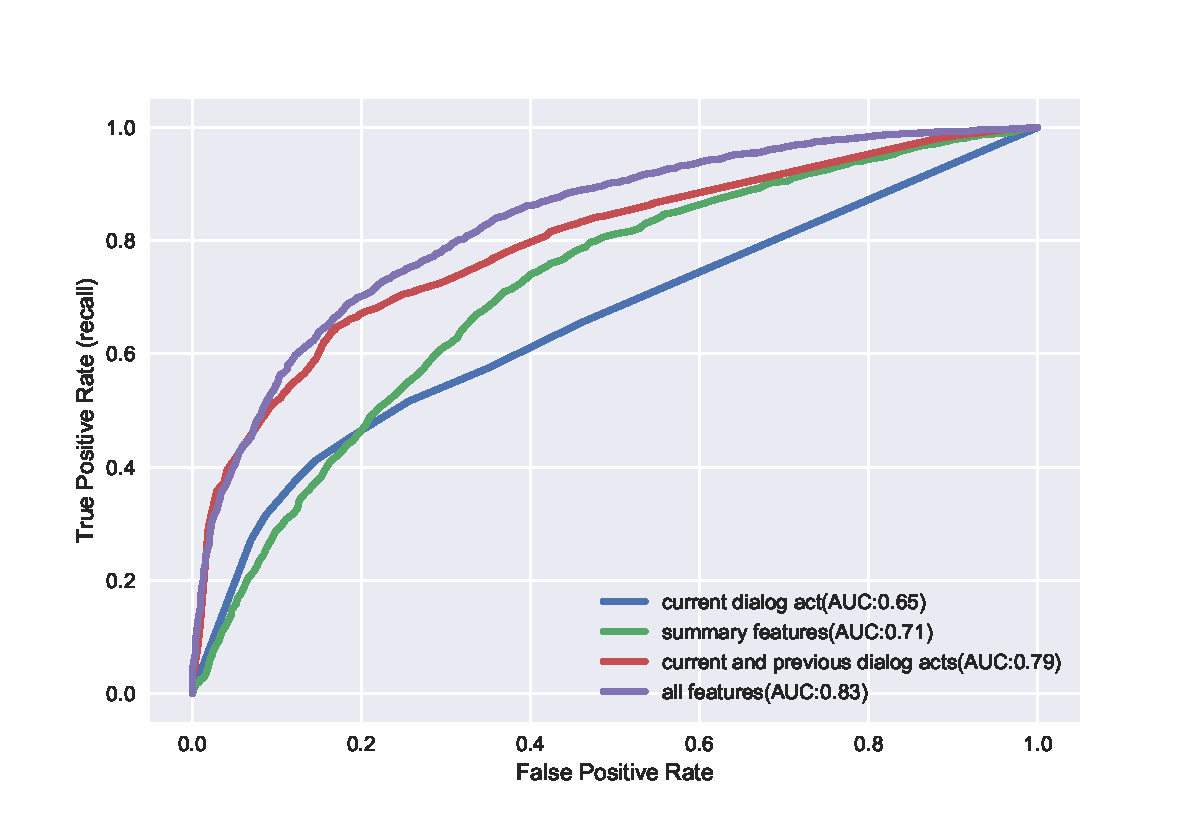
\includegraphics[width=32em]{../scikitlearn/figures/roc.pdf}
 \end{figure}
\end{frame}


\begin{frame} {Sensitivity to Measurement Start Time}
\begin{table}
\begin{center}
\begin{tabular}{lrrrrrrr}
\hline
{} & 0s & 15s & 30s & 45s & 60s & {\bf 120s} & 180s  \\
\hline
baseline 1 & 65.99\% & 66.10\% & 66.12\% & 66.09\%  & 66.02\% & 65.98\% & 66.05\%  \\
baseline 2 & 81.11\% & 81.21\% & 81.24\% & 81.20\%  & 81.15\% & 80.92\% & 80.68\%  \\
summary    & 69.46\% & 69.51\% & 69.43\% & 69.49\%  & 69.57\% & 69.10\% & 69.21\%  \\
full       & 83.78\% & 83.87\% & 83.85\% & 83.80\%  & 83.61\% & 83.19\% & 82.80\%  \\
\hline
\end{tabular}
\end{center}
\caption{ AUC Score in relation to the start of the dialog }
\label{table:starttime}
\end{table}

\end{frame}{}

`% !TeX root = ../defense.tex

\section{Summary}
\frame{\sectionpage}

\begin{frame}{Conclusion}
   \begin{enumerate}[<+->]\itemsep9pt
      \item Summary features do provide improvement over local features. 
      \item However, the affect for our data is the opposite of our initial assumption
              \begin{itemize}
                \item Short turn (Low RTL) leads to turn change
                \item In long turn the speaker will actually hold the floor.
               \end{itemize}
    \end{enumerate}
\end{frame}{}

\begin{frame}{Future work}
   \begin{enumerate}[<+->]\itemsep9pt
      \item Combine the summary features with other local features (semantic/prosadic)
      \item Test the hypothesis on another type of corpus (for example task based corpus)
      \item Instead of measuring the affect from the start of the conversation, use moving averages with different window length.
      \item Perform the experiments where back channels are not considered as turn change. 
      \item In general, any local features can be turned into a summary feature by taking the avarage
            over past turn. Hence this area of research can be expanded to other local features.
      
          
    \end{enumerate}
\end{frame}{}



\begin{frame} {Acknowledgement}
 \begin{center}
       \begin{enumerate}[<+->]\itemsep9pt
           \item This work was partially funded by the National Science Foundation under grant IIS-1321146.
           \item This thesis is based on a paper that was submitted and presented at Interspeech 2016.
           \item Thesis advisor and collaborator : Prof. Peter Heeman.
       \end{enumerate}
 \end{center}
\end{frame}



%\bibliographystyle{abbrv} % check with your advisor for appropriate style
%\bibliography{thesis} % name of your thesis.bib file

%\begin{frame} {References}
% This prints the bibliography on the slide
%\printbibliography
%\end{frame}


\end{document}
